% -*- coding: utf-8 -*-
% (картинка справа от куска кода с циклическими парами)

% Отключить костыли для генератора картинок
\ifPreview\else\begin{float:right}\correct{0.25em}{-1.0em}\fi

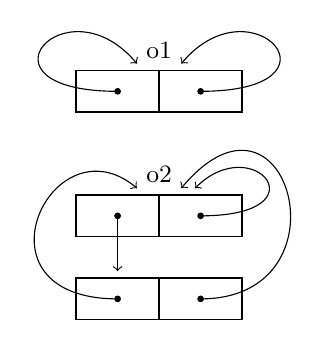
\begin{tikzpicture}
  \clip (-1.75em,-0.25em) rectangle (8.00em, 10.55em);

% o2
  \draw [semithick] (0.0em, 0.0em) rectangle (6.0em, 1.5em);
  \draw [semithick] (3.0em, 0.0em) -- (3.0em, 1.5em);
  \draw [semithick] (0.0em, 3.0em) rectangle (6.0em, 4.5em);
  \draw [semithick] (3.0em, 3.0em) -- (3.0em, 4.5em);

  \draw [->] (1.5em, 0.75em) .. controls +(180:5.5em) and +(140:4.0em) .. (2.2em, 4.75em);
  \draw [->] (4.5em, 0.75em) .. controls +(  0:5.5em) and +( 50:6.0em) .. (3.8em, 4.75em);
  \draw [->] (4.5em, 3.75em) .. controls +(  0:4.5em) and +( 45:3.0em) .. (4.3em, 4.75em);
  \draw [->] (1.5em, 3.75em) -- (1.5em, 1.75em);

  \filldraw  (1.5em, 0.75em) circle(1.0pt);
  \filldraw  (4.5em, 0.75em) circle(1.0pt);
  \filldraw  (1.5em, 3.75em) circle(1.0pt);
  \filldraw  (4.5em, 3.75em) circle(1.0pt);

% o1
  \draw [semithick] (0.0em, 7.5em) rectangle (6.0em, 9.0em);
  \draw [semithick] (3.0em, 7.5em) -- (3.0em, 9.0em);

  \draw [->] (1.5em, 8.25em) .. controls +(180:5.5em) and +(130:4.0em) .. (2.2em, 9.25em);
  \draw [->] (4.5em, 8.25em) .. controls +(  0:5.5em) and +( 50:4.0em) .. (3.8em, 9.25em);

  \filldraw  (1.5em, 8.25em) circle(1.0pt);
  \filldraw  (4.5em, 8.25em) circle(1.0pt);


  \draw (3.0em, 4.6em) node[above] {\small\ic{o2}};
  \draw (3.0em, 9.1em) node[above] {\small\ic{o1}};

\end{tikzpicture}

\ifPreview\else\end{float:right}\fi
